\documentclass[aspectratio=169]{beamer}

% Minimal theme
\usetheme{default}
\usecolortheme{dove}

% Remove navigation symbols
\setbeamertemplate{navigation symbols}{}
\setbeamertemplate{footline}{%
  \hfill{\large\insertframenumber\,/\,\inserttotalframenumber}\hspace{0.8em}\vspace{0.5em}%
}

% Colors
\definecolor{popblue}{RGB}{52, 101, 164}
\definecolor{sampred}{RGB}{204, 0, 0}
\definecolor{paramgreen}{RGB}{0, 140, 70}
\definecolor{lightbg}{RGB}{245, 245, 250}
\definecolor{warnred}{RGB}{180, 40, 40}
\definecolor{orange1}{RGB}{220, 120, 0}
\definecolor{violet1}{RGB}{120, 50, 160}

\setbeamercolor{frametitle}{fg=popblue}
\setbeamercolor{title}{fg=popblue}

% Packages
\usepackage{pgfplots}
\usepackage{tikz}
\usetikzlibrary{shapes, arrows.meta, positioning, calc, decorations.pathreplacing, patterns}
\pgfplotsset{compat=1.18}
\usepackage{amsmath, amssymb}
\usepackage{fontenc}

\title{Lecture 1: Foundations}
\subtitle{Probability vs Statistics $\cdot$ Population \& Sample $\cdot$ i.i.d. $\cdot$ Plug-in Principle $\cdot$ Loss \& Risk}
\date{}

\begin{document}

% ============================================================
% TITLE
% ============================================================
\begin{frame}
\titlepage
\end{frame}

% ============================================================
% MOTIVATING QUESTION
% ============================================================
\begin{frame}
\frametitle{How much should you trust a number?}

\begin{center}
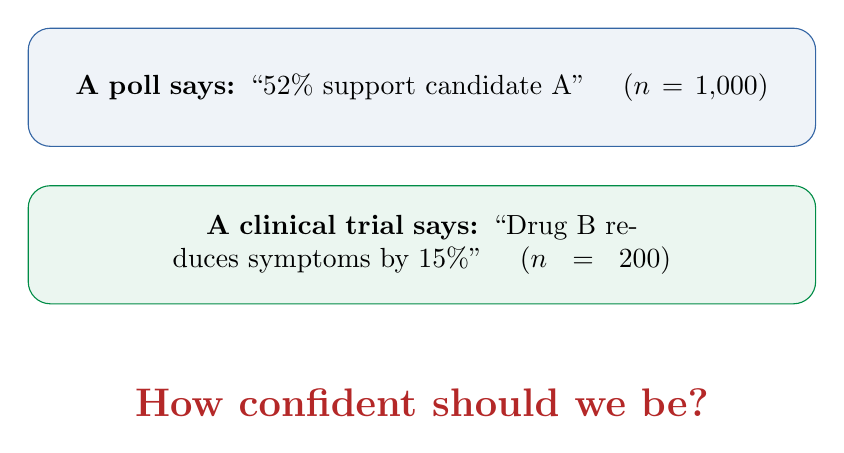
\begin{tikzpicture}
  % Poll box
  \node[draw=popblue, fill=popblue!8, rounded corners=8pt, minimum width=10cm, minimum height=1.5cm, text width=9.5cm, align=center] at (0, 1.5) {
    \textbf{A poll says:} ``52\% support candidate A'' \quad ($n = 1{,}000$)
  };
  % Trial box
  \node[draw=paramgreen, fill=paramgreen!8, rounded corners=8pt, minimum width=10cm, minimum height=1.5cm, text width=9.5cm, align=center] at (0, -0.5) {
    \textbf{A clinical trial says:} ``Drug B reduces symptoms by 15\%'' \quad ($n = 200$)
  };
  % Question
  \node[font=\Large\bfseries, text=warnred] at (0, -2.5) {How confident should we be?};
\end{tikzpicture}
\end{center}

\vspace{0.3cm}
This entire course is about answering this question rigorously.
\end{frame}

% ============================================================
% 0.1 PROBABILITY VS STATISTICS
% ============================================================
\section{Probability vs Statistics}

\begin{frame}
\frametitle{Probability vs Statistics}
\begin{center}
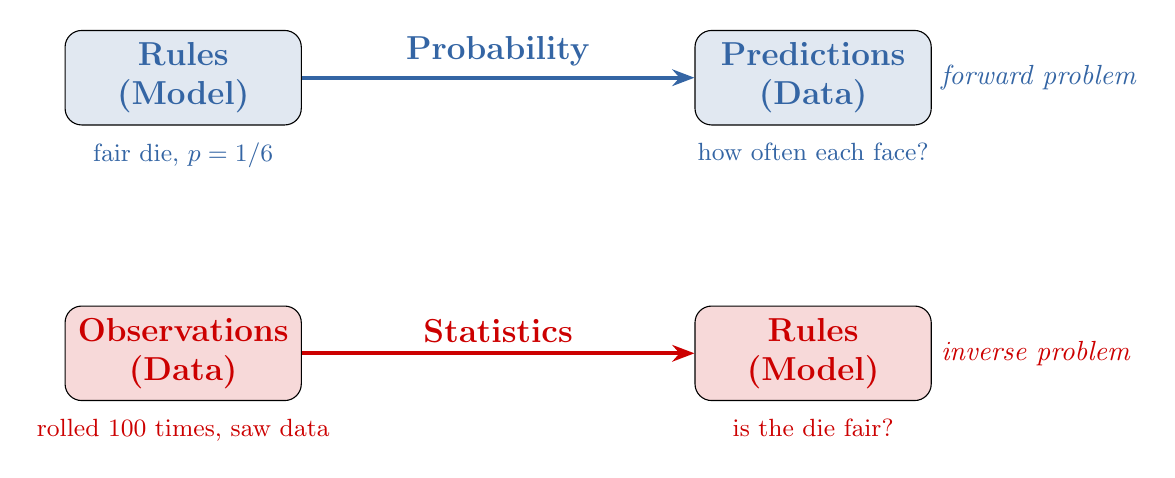
\begin{tikzpicture}[
  box/.style={draw, rounded corners=6pt, minimum width=3cm, minimum height=1.2cm, font=\large\bfseries, align=center},
  arrow/.style={-{Stealth[length=8pt]}, line width=1.5pt}
]
  % Probability side
  \node[box, fill=popblue!15, text=popblue] (rules) at (-4, 2) {Rules\\(Model)};
  \node[box, fill=popblue!15, text=popblue] (data1) at (4, 2) {Predictions\\(Data)};
  \draw[arrow, popblue] (rules) -- (data1) node[midway, above, font=\large] {\textbf{Probability}};
  \node[font=\small, text=popblue, below=0.1cm of rules] {fair die, $p=1/6$};
  \node[font=\small, text=popblue, below=0.1cm of data1] {how often each face?};

  % Statistics side
  \node[box, fill=sampred!15, text=sampred] (data2) at (-4, -1.5) {Observations\\(Data)};
  \node[box, fill=sampred!15, text=sampred] (model) at (4, -1.5) {Rules\\(Model)};
  \draw[arrow, sampred] (data2) -- (model) node[midway, above, font=\large] {\textbf{Statistics}};
  \node[font=\small, text=sampred, below=0.1cm of data2] {rolled 100 times, saw data};
  \node[font=\small, text=sampred, below=0.1cm of model] {is the die fair?};

  % Labels
  \node[font=\normalsize, popblue, right] at (5.5, 2) {\textit{forward problem}};
  \node[font=\normalsize, sampred, right] at (5.5, -1.5) {\textit{inverse problem}};
\end{tikzpicture}
\end{center}
\end{frame}

\begin{frame}
\frametitle{Why the inverse problem is harder}
\begin{center}
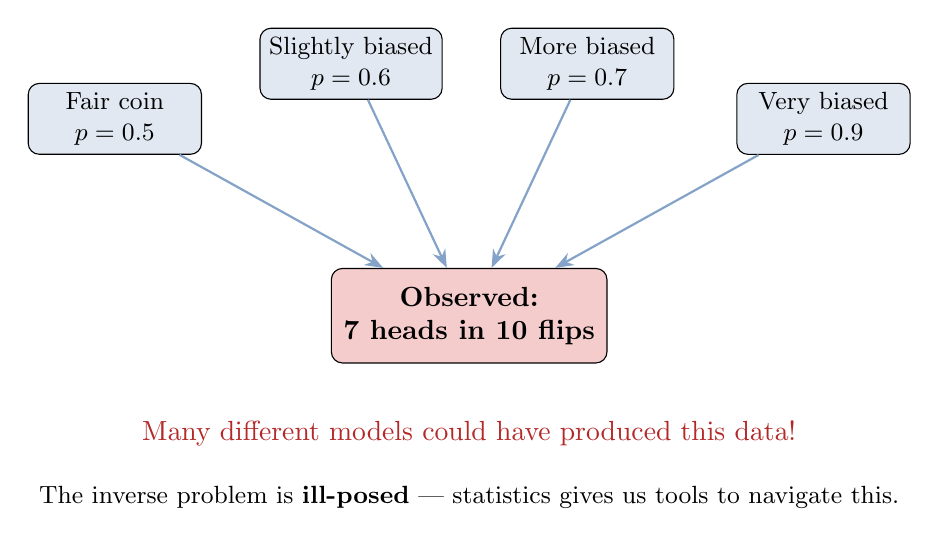
\begin{tikzpicture}[
  box/.style={draw, rounded corners=4pt, minimum width=2.2cm, minimum height=0.9cm, font=\small, align=center}
]
  % Data in center
  \node[box, fill=sampred!20, font=\normalsize\bfseries, minimum width=3.5cm, minimum height=1.2cm] (data) at (0, 0) {Observed:\\7 heads in 10 flips};

  % Multiple models
  \node[box, fill=popblue!15] (m1) at (-4.5, 2.5) {Fair coin\\$p = 0.5$};
  \node[box, fill=popblue!15] (m2) at (-1.5, 3.2) {Slightly biased\\$p = 0.6$};
  \node[box, fill=popblue!15] (m3) at (1.5, 3.2) {More biased\\$p = 0.7$};
  \node[box, fill=popblue!15] (m4) at (4.5, 2.5) {Very biased\\$p = 0.9$};

  % Arrows from models to data
  \draw[-{Stealth}, thick, popblue!60] (m1) -- (data);
  \draw[-{Stealth}, thick, popblue!60] (m2) -- (data);
  \draw[-{Stealth}, thick, popblue!60] (m3) -- (data);
  \draw[-{Stealth}, thick, popblue!60] (m4) -- (data);

  % Question
  \node[font=\normalsize, text=warnred] at (0, -1.5) {Many different models could have produced this data!};
  \node[font=\small] at (0, -2.3) {The inverse problem is \textbf{ill-posed} --- statistics gives us tools to navigate this.};
\end{tikzpicture}
\end{center}
\end{frame}

% ============================================================
% 0.2 POPULATION, SAMPLE, PARAMETER, STATISTIC
% ============================================================
\section{Population, Sample, Parameter, Statistic}

\begin{frame}
\frametitle{Population vs Sample}
\begin{center}
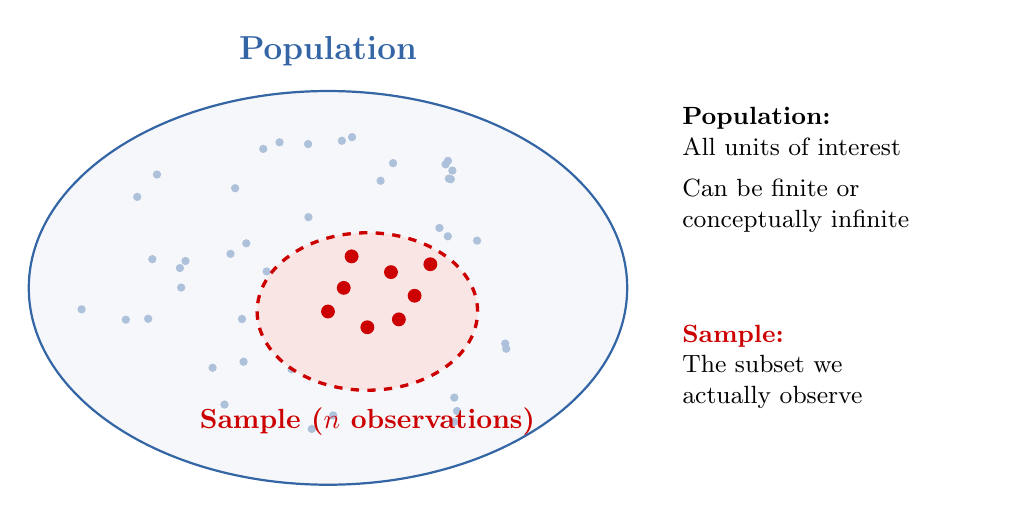
\begin{tikzpicture}
  % Population - large circle with many dots
  \draw[thick, popblue, fill=popblue!5] (0,0) ellipse (3.8cm and 2.5cm);
  \node[font=\large\bfseries, popblue] at (0, 3) {Population};

  % Random dots in population
  \foreach \i in {1,...,80} {
    \pgfmathsetmacro{\rx}{3.5*rand}
    \pgfmathsetmacro{\ry}{2.2*rand}
    \pgfmathparse{(\rx/3.5)^2 + (\ry/2.2)^2 < 0.85 ? 1 : 0}
    \ifnum\pgfmathresult=1
      \fill[popblue!40] (\rx, \ry) circle (1.5pt);
    \fi
  }

  % Sample - highlighted subset
  \draw[very thick, sampred, fill=sampred!10, dashed] (0.5, -0.3) ellipse (1.4cm and 1cm);
  \node[font=\bfseries, sampred] at (0.5, -1.7) {Sample ($n$ observations)};

  % Red dots in sample
  \foreach \x/\y in {0.2/0, 0.8/0.2, 0.5/-0.5, 1.1/-0.1, 0.3/0.4, 0.9/-0.4, 0/-0.3, 1.3/0.3} {
    \fill[sampred] (\x, \y) circle (2.5pt);
  }

  % Annotations
  \node[text width=4cm, align=left, font=\small] at (6.5, 1.5) {
    \textbf{Population:}\\
    All units of interest\\[4pt]
    Can be finite or\\
    conceptually infinite
  };
  \node[text width=4cm, align=left, font=\small] at (6.5, -1) {
    \textcolor{sampred}{\textbf{Sample:}}\\
    The subset we\\
    actually observe
  };
\end{tikzpicture}
\end{center}
\end{frame}

\begin{frame}
\frametitle{Parameter vs Statistic}
\begin{center}
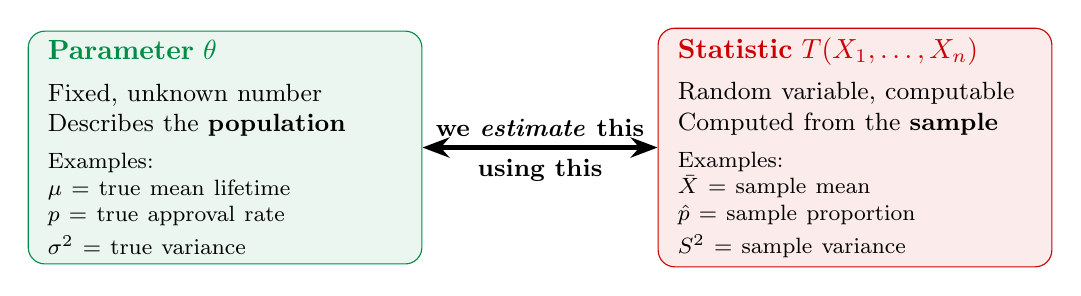
\begin{tikzpicture}[
  parambox/.style={draw=paramgreen, fill=paramgreen!8, rounded corners=6pt, minimum width=5cm, minimum height=2.5cm, text width=4.5cm, align=left},
  statbox/.style={draw=sampred, fill=sampred!8, rounded corners=6pt, minimum width=5cm, minimum height=2.5cm, text width=4.5cm, align=left}
]
  \node[parambox] (param) at (-4, 0) {
    \textbf{\textcolor{paramgreen}{Parameter $\theta$}}\\[4pt]
    \small Fixed, unknown number\\
    Describes the \textbf{population}\\[4pt]
    \footnotesize Examples:\\
    \footnotesize $\mu$ = true mean lifetime\\
    \footnotesize $p$ = true approval rate\\
    \footnotesize $\sigma^2$ = true variance
  };
  \node[statbox] (stat) at (4, 0) {
    \textbf{\textcolor{sampred}{Statistic $T(X_1, \ldots, X_n)$}}\\[4pt]
    \small Random variable, computable\\
    Computed from the \textbf{sample}\\[4pt]
    \footnotesize Examples:\\
    \footnotesize $\bar{X}$ = sample mean\\
    \footnotesize $\hat{p}$ = sample proportion\\
    \footnotesize $S^2$ = sample variance
  };

  % Key distinction
  \draw[{Stealth}-{Stealth}, thick, line width=1.5pt] (param) -- (stat)
    node[midway, above, font=\small\bfseries] {we \textit{estimate} this}
    node[midway, below, font=\small\bfseries] {using this};
\end{tikzpicture}
\end{center}

\vspace{0.3cm}
\begin{center}
\fcolorbox{warnred}{warnred!5}{%
  \parbox{10cm}{\centering\small
    A \textbf{parameter} is a fixed number. A \textbf{statistic} is a random variable.\\
    Confusing these is the source of most beginner mistakes.
  }%
}
\end{center}
\end{frame}

\begin{frame}
\frametitle{The Triple: Estimand / Estimator / Estimate}
\begin{center}
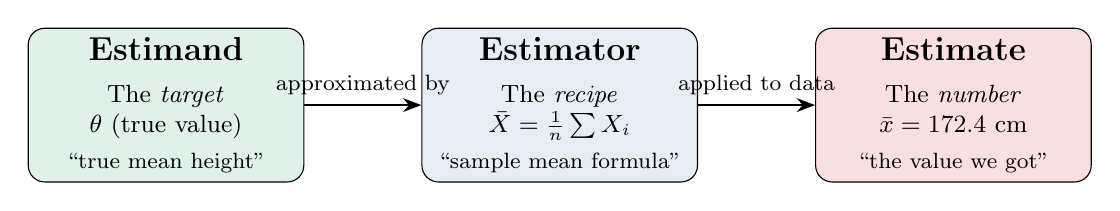
\begin{tikzpicture}[
  tribox/.style={draw, rounded corners=6pt, minimum width=3.5cm, minimum height=1.8cm, align=center, font=\small}
]
  \node[tribox, fill=paramgreen!12] (estimand) at (-5, 0) {
    \textbf{\large Estimand}\\[4pt]
    The \textit{target}\\
    $\theta$ (true value)\\[2pt]
    \footnotesize ``true mean height''
  };
  \node[tribox, fill=popblue!12] (estimator) at (0, 0) {
    \textbf{\large Estimator}\\[4pt]
    The \textit{recipe}\\
    $\bar{X} = \frac{1}{n}\sum X_i$\\[2pt]
    \footnotesize ``sample mean formula''
  };
  \node[tribox, fill=sampred!12] (estimate) at (5, 0) {
    \textbf{\large Estimate}\\[4pt]
    The \textit{number}\\
    $\bar{x} = 172.4$ cm\\[2pt]
    \footnotesize ``the value we got''
  };

  \draw[-{Stealth}, thick] (estimand) -- (estimator) node[midway, above, font=\footnotesize] {approximated by};
  \draw[-{Stealth}, thick] (estimator) -- (estimate) node[midway, above, font=\footnotesize] {applied to data};
\end{tikzpicture}
\end{center}
\end{frame}

\begin{frame}
\frametitle{Discussion}
\begin{center}
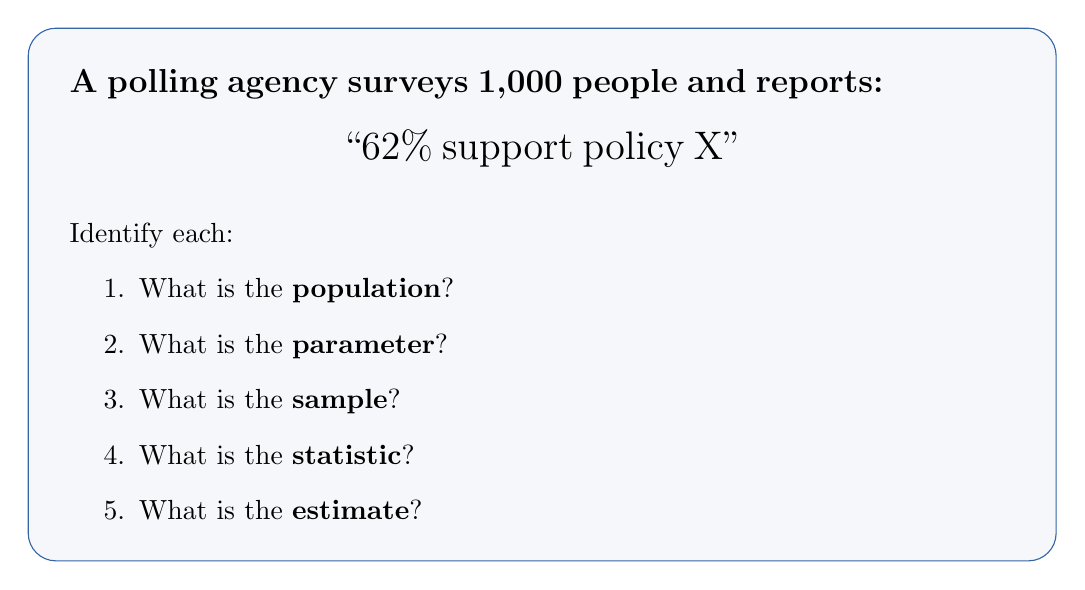
\begin{tikzpicture}
  \node[draw=popblue, fill=popblue!5, rounded corners=10pt, text width=12cm, align=left, inner sep=15pt] {
    \textbf{\large A polling agency surveys 1{,}000 people and reports:}\\[8pt]
    \begin{center}
    {\Large ``62\% support policy X''}
    \end{center}
    \vspace{8pt}
    Identify each:
    \begin{enumerate}
      \item What is the \textbf{population}?
      \item What is the \textbf{parameter}?
      \item What is the \textbf{sample}?
      \item What is the \textbf{statistic}?
      \item What is the \textbf{estimate}?
    \end{enumerate}
  };
\end{tikzpicture}
\end{center}
\end{frame}

\begin{frame}
\frametitle{Discussion: Answers}
\begin{center}
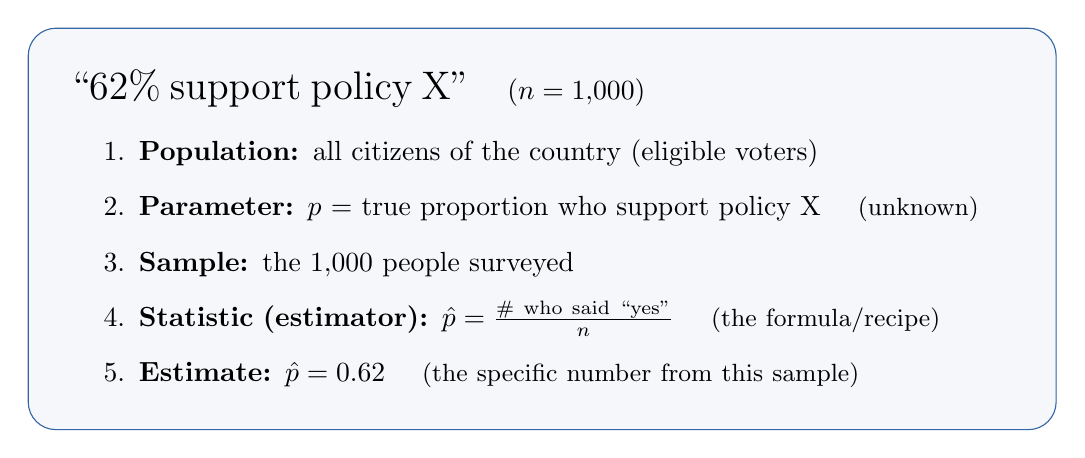
\begin{tikzpicture}
  \node[draw=popblue, fill=popblue!5, rounded corners=10pt, text width=12cm, align=left, inner sep=15pt] {
    {\Large ``62\% support policy X''} \quad ($n = 1{,}000$)\\[10pt]
    \begin{enumerate}
      \item \textbf{Population:} all citizens of the country (eligible voters)
      \item \textbf{Parameter:} $p$ = true proportion who support policy X \quad {\small (unknown)}
      \item \textbf{Sample:} the 1{,}000 people surveyed
      \item \textbf{Statistic (estimator):} $\hat{p} = \frac{\text{\# who said ``yes''}}{n}$ \quad {\small (the formula/recipe)}
      \item \textbf{Estimate:} $\hat{p} = 0.62$ \quad {\small (the specific number from this sample)}
    \end{enumerate}
  };
\end{tikzpicture}
\end{center}
\end{frame}

% ============================================================
% 0.3 THE I.I.D. ASSUMPTION
% ============================================================
\section{The i.i.d. Assumption}

\begin{frame}
\frametitle{The i.i.d. Assumption}

Classical statistics assumes our sample $X_1, X_2, \ldots, X_n$ is \textbf{i.i.d.}:

\vspace{0.4cm}
\begin{center}
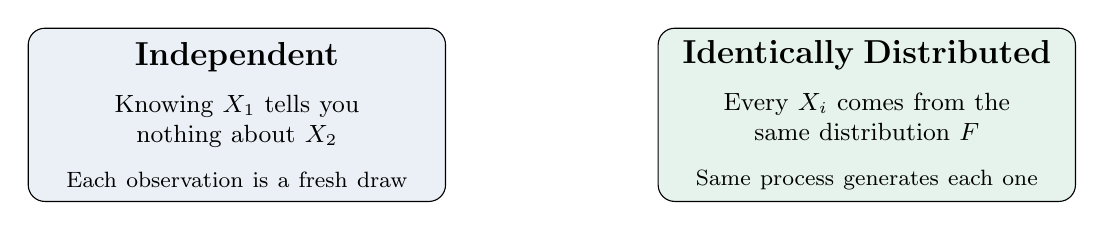
\begin{tikzpicture}[
  iidbox/.style={draw, rounded corners=6pt, minimum width=5.3cm, minimum height=2.2cm, align=center, text width=5cm}
]
  \node[iidbox, fill=popblue!10] at (-4, 0) {
    \textbf{\large Independent}\\[6pt]
    \small Knowing $X_1$ tells you\\
    nothing about $X_2$\\[4pt]
    \footnotesize Each observation is a fresh draw
  };
  \node[iidbox, fill=paramgreen!10] at (4, 0) {
    \textbf{\large Identically Distributed}\\[6pt]
    \small Every $X_i$ comes from the\\
    same distribution $F$\\[4pt]
    \footnotesize Same process generates each one
  };
\end{tikzpicture}
\end{center}
\end{frame}

\begin{frame}
\frametitle{When does i.i.d. hold?}
\begin{center}
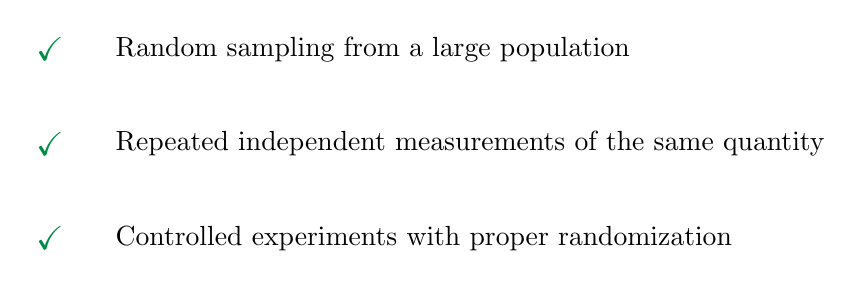
\begin{tikzpicture}
  % Check marks with examples
  \foreach \y/\txt in {
    2/{Random sampling from a large population},
    0.8/{Repeated independent measurements of the same quantity},
    -0.4/{Controlled experiments with proper randomization}
  } {
    \node[font=\large, paramgreen] at (-5.5, \y) {\checkmark};
    \node[anchor=west, font=\normalsize] at (-4.8, \y) {\txt};
  }
\end{tikzpicture}
\end{center}

\vspace{0.5cm}
\begin{center}
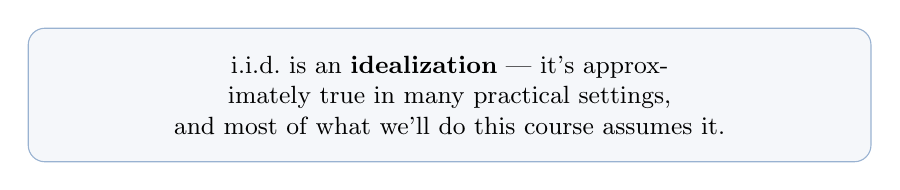
\begin{tikzpicture}
  \node[draw=popblue!50, fill=popblue!5, rounded corners=6pt, text width=10cm, align=center, inner sep=10pt, font=\small] {
    i.i.d.\ is an \textbf{idealization} --- it's approximately true in many practical settings,\\
    and most of what we'll do this course assumes it.
  };
\end{tikzpicture}
\end{center}
\end{frame}

\begin{frame}
\frametitle{When does i.i.d. break?}
\begin{center}
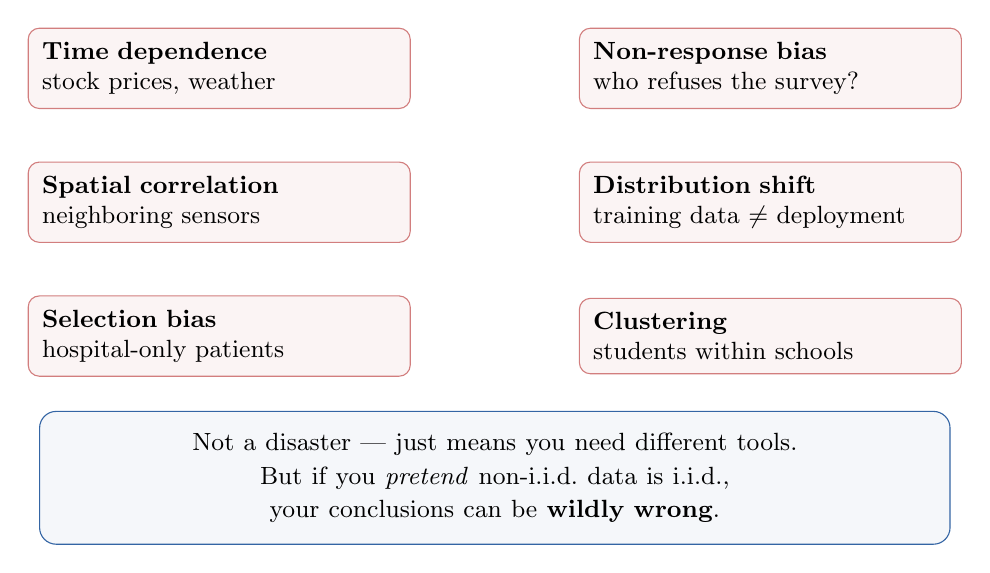
\begin{tikzpicture}[
  failbox/.style={draw=warnred!60, fill=warnred!5, rounded corners=4pt, minimum height=0.9cm, text width=4.5cm, align=left, font=\small, inner sep=5pt}
]
  % Left column
  \node[failbox] at (-3.5, 2.5) {\textbf{Time dependence}\\stock prices, weather};
  \node[failbox] at (-3.5, 0.8) {\textbf{Spatial correlation}\\neighboring sensors};
  \node[failbox] at (-3.5, -0.9) {\textbf{Selection bias}\\hospital-only patients};

  % Right column
  \node[failbox] at (3.5, 2.5) {\textbf{Non-response bias}\\who refuses the survey?};
  \node[failbox] at (3.5, 0.8) {\textbf{Distribution shift}\\training data $\ne$ deployment};
  \node[failbox] at (3.5, -0.9) {\textbf{Clustering}\\students within schools};

  % Bottom message
  \node[draw=popblue, fill=popblue!5, rounded corners=6pt, text width=11cm, align=center, inner sep=8pt] at (0, -2.7) {
    \small Not a disaster --- just means you need different tools.\\
    But if you \textit{pretend} non-i.i.d.\ data is i.i.d., your conclusions can be \textbf{wildly wrong}.
  };
\end{tikzpicture}
\end{center}
\end{frame}

\begin{frame}
\frametitle{Survivorship Bias}
\begin{columns}[T]
\begin{column}{0.38\textwidth}
  \begin{center}
    \includegraphics[width=\columnwidth, height=5.5cm, keepaspectratio]{survivorship_airplane.pdf}
  \end{center}
\end{column}
\begin{column}{0.58\textwidth}
  \small
  \textbf{WW2:} Engineers studied bullet holes on returning bombers and proposed armoring the hit areas.

  \vspace{0.2cm}
  Abraham Wald: \textit{``You're only seeing planes that \textbf{survived}. Armor the places with \textbf{no} holes --- those hits brought planes down.''}

  \vspace{0.3cm}
  \textbf{More examples:}
  \begin{itemize}\setlength{\itemsep}{2pt}
    \item Online survey: ``Do you have internet?'' --- 100\% say yes
    \item ``Soviet products lasted forever'' --- you only see the ones that survived
    \item Bus fare survey: asking people \textit{on the bus} ``100$\to$150 AMD?'' --- only sampling current riders
  \end{itemize}
\end{column}
\end{columns}
\end{frame}

% ============================================================
% 0.4 THE PLUG-IN PRINCIPLE
% ============================================================
\section{The Plug-in Principle}

\begin{frame}
\frametitle{The Plug-in Principle}

\textbf{Idea:} We don't know the true distribution $F$, so replace it with the \textbf{empirical distribution} $\hat{F}_n$.

\vspace{0.3cm}
\begin{center}
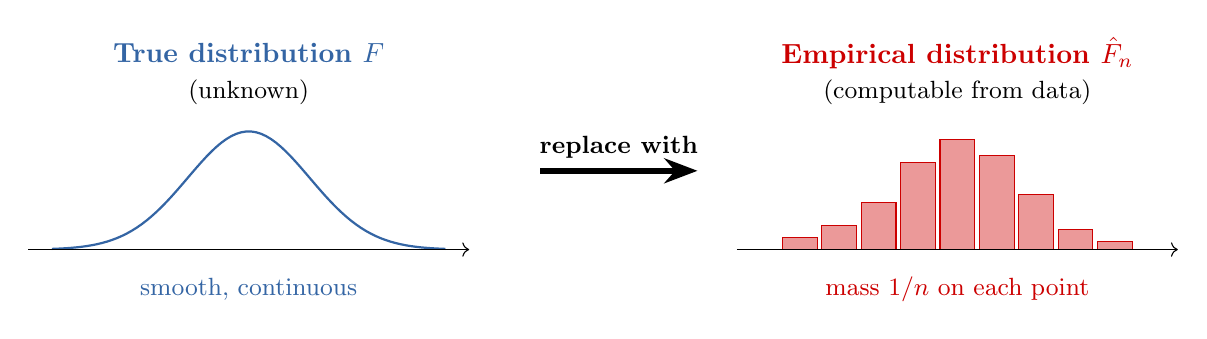
\begin{tikzpicture}
  % True distribution
  \begin{scope}[xshift=-4.5cm]
    \node[font=\bfseries, popblue] at (0, 2.5) {True distribution $F$};
    \node[font=\small] at (0, 2) {(unknown)};
    \draw[thick, popblue, domain=-2.5:2.5, samples=80] plot (\x, {1.5*exp(-\x*\x/1.2)});
    \draw[->] (-2.8, 0) -- (2.8, 0);
    \node[font=\small, popblue] at (0, -0.5) {smooth, continuous};
  \end{scope}

  % Arrow
  \draw[-{Stealth}, very thick, line width=2pt] (-0.8, 1) -- (1.2, 1)
    node[midway, above, font=\small\bfseries] {replace with};

  % Empirical distribution
  \begin{scope}[xshift=4.5cm]
    \node[font=\bfseries, sampred] at (0, 2.5) {Empirical distribution $\hat{F}_n$};
    \node[font=\small] at (0, 2) {(computable from data)};
    % Histogram-like bars
    \foreach \x/\h in {-2/0.15, -1.5/0.3, -1/0.6, -0.5/1.1, 0/1.4, 0.5/1.2, 1/0.7, 1.5/0.25, 2/0.1} {
      \fill[sampred!40] (\x-0.22, 0) rectangle (\x+0.22, \h);
      \draw[sampred] (\x-0.22, 0) rectangle (\x+0.22, \h);
    }
    \draw[->] (-2.8, 0) -- (2.8, 0);
    \node[font=\small, sampred] at (0, -0.5) {mass $1/n$ on each point};
  \end{scope}
\end{tikzpicture}
\end{center}
\end{frame}

\begin{frame}
\frametitle{Plug-in in Action}

Replace the \textbf{population quantity} with its \textbf{sample analogue}:

\vspace{0.5cm}
\renewcommand{\arraystretch}{1.8}
\begin{center}
\begin{tabular}{lcc}
  \textbf{Want} & \textbf{Population} & \textbf{Plug-in} \\
  \hline
  Mean & $\mu = \mathbb{E}_F[X]$ & $\hat{\mu} = \bar{X} = \frac{1}{n}\sum X_i$ \\[4pt]
  Variance & $\sigma^2 = \text{Var}_F(X)$ & $\hat{\sigma}^2 = \frac{1}{n}\sum (X_i - \bar{X})^2$ \\[4pt]
  CDF & $F(t) = P(X \le t)$ & $\hat{F}_n(t) = \frac{\#\{X_i \le t\}}{n}$ \\
  \hline
\end{tabular}
\end{center}

\vspace{0.4cm}
\textbf{Glivenko--Cantelli theorem:} $\hat{F}_n \to F$ uniformly as $n \to \infty$.

\small (The ``fundamental theorem of statistics'' --- connects to LLN from Module 20.)
\end{frame}

% ============================================================
% 0.5 LOSS, RISK, OPTIMAL SUMMARIES
% ============================================================
\section{Loss, Risk, and Optimal Summaries}

\begin{frame}
\frametitle{The Summarization Problem}

\begin{center}
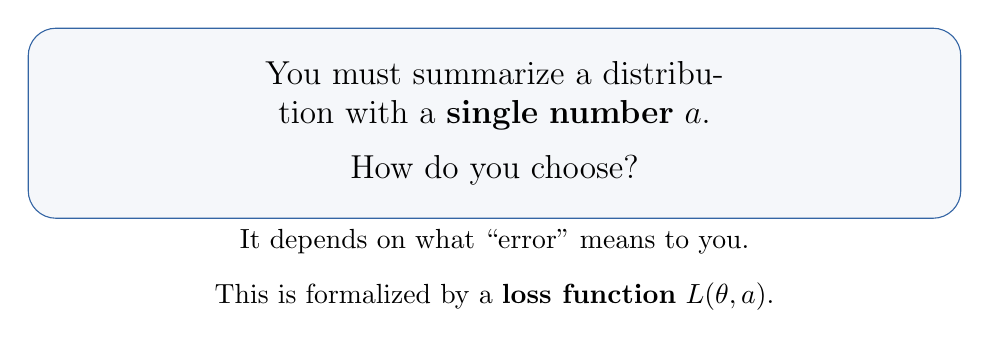
\begin{tikzpicture}
  \node[draw=popblue, fill=popblue!5, rounded corners=10pt, text width=11cm, align=center, inner sep=12pt, font=\large] {
    You must summarize a distribution with a \textbf{single number} $a$.\\[6pt]
    How do you choose?
  };

  \node[font=\normalsize] at (0, -1.5) {It depends on what ``error'' means to you.};
  \node[font=\normalsize] at (0, -2.2) {This is formalized by a \textbf{loss function} $L(\theta, a)$.};
\end{tikzpicture}
\end{center}
\end{frame}

\begin{frame}
\frametitle{Three Losses, Three Optimal Summaries}
\begin{center}
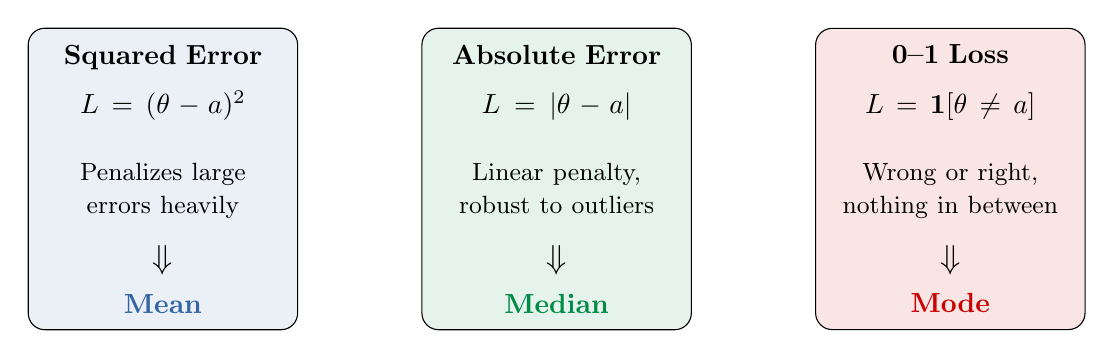
\begin{tikzpicture}[
  lossbox/.style={draw, rounded corners=6pt, minimum width=3.3cm, minimum height=3.5cm, align=center, text width=3cm, inner sep=6pt}
]
  % Squared error
  \node[lossbox, fill=popblue!10] (sq) at (-5, 0) {
    \textbf{Squared Error}\\[6pt]
    $L = (\theta - a)^2$\\[12pt]
    {\small Penalizes large}\\
    {\small errors heavily}\\[8pt]
    \textbf{\large $\Downarrow$}\\[4pt]
    \textcolor{popblue}{\textbf{Mean}}
  };

  % Absolute error
  \node[lossbox, fill=paramgreen!10] (abs) at (0, 0) {
    \textbf{Absolute Error}\\[6pt]
    $L = |\theta - a|$\\[12pt]
    {\small Linear penalty,}\\
    {\small robust to outliers}\\[8pt]
    \textbf{\large $\Downarrow$}\\[4pt]
    \textcolor{paramgreen}{\textbf{Median}}
  };

  % 0-1 loss
  \node[lossbox, fill=sampred!10] (zo) at (5, 0) {
    \textbf{0--1 Loss}\\[6pt]
    $L = \mathbf{1}[\theta \ne a]$\\[12pt]
    {\small Wrong or right,}\\
    {\small nothing in between}\\[8pt]
    \textbf{\large $\Downarrow$}\\[4pt]
    \textcolor{sampred}{\textbf{Mode}}
  };
\end{tikzpicture}
\end{center}
\end{frame}

\begin{frame}
\frametitle{Visualizing the Losses}
\begin{center}
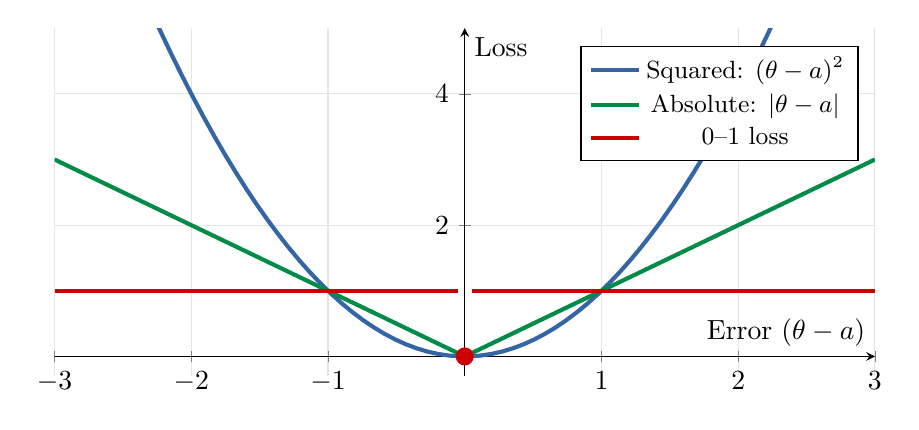
\begin{tikzpicture}
  \begin{axis}[
    width=12cm, height=6cm,
    xlabel={Error ($\theta - a$)},
    ylabel={Loss},
    xmin=-3, xmax=3,
    ymin=-0.3, ymax=5,
    axis lines=middle,
    legend style={at={(0.98,0.95)}, anchor=north east, font=\small},
    grid=major,
    grid style={gray!20},
    every axis plot/.append style={line width=1.5pt}
  ]
    % Squared error
    \addplot[popblue, domain=-2.3:2.3, samples=60] {x^2};
    \addlegendentry{Squared: $(\theta-a)^2$}

    % Absolute error
    \addplot[paramgreen, domain=-3:3, samples=60] {abs(x)};
    \addlegendentry{Absolute: $|\theta-a|$}

    % 0-1 loss (approximated with step)
    \addplot[sampred, domain=-3:-0.05, samples=30] {1};
    \addplot[sampred, domain=0.05:3, samples=30, forget plot] {1};
    \addplot[sampred, only marks, mark=*, mark size=2.5pt, forget plot] coordinates {(0,0)};
    \addlegendentry{0--1 loss}
  \end{axis}
\end{tikzpicture}
\end{center}
\end{frame}

\begin{frame}
\frametitle{Mean vs Median: Sensitivity to Outliers}
\begin{center}
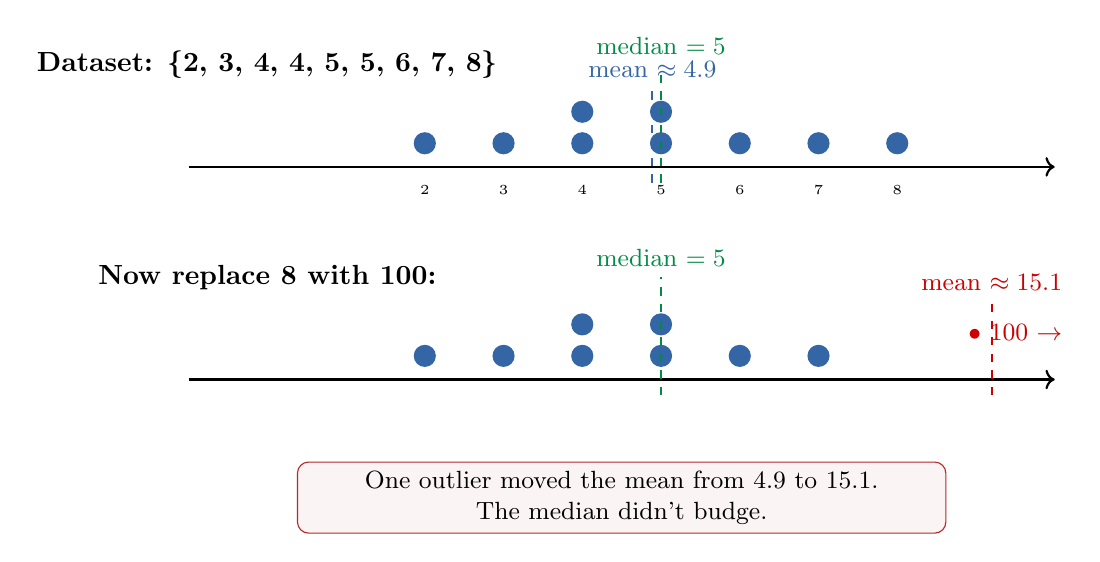
\begin{tikzpicture}
  % Dataset 1: no outlier
  \node[font=\bfseries] at (0, 3.5) {Dataset: \{2, 3, 4, 4, 5, 5, 6, 7, 8\}};

  % Dot plot 1
  \draw[thick, ->] (-1, 2.2) -- (10, 2.2);
  \foreach \x in {2,3,4,5,6,7,8} {
    \node[font=\tiny] at (\x, 1.9) {\x};
  }
  \fill[popblue] (2, 2.5) circle (4pt);
  \fill[popblue] (3, 2.5) circle (4pt);
  \fill[popblue] (4, 2.5) circle (4pt);
  \fill[popblue] (4, 2.9) circle (4pt);
  \fill[popblue] (5, 2.5) circle (4pt);
  \fill[popblue] (5, 2.9) circle (4pt);
  \fill[popblue] (6, 2.5) circle (4pt);
  \fill[popblue] (7, 2.5) circle (4pt);
  \fill[popblue] (8, 2.5) circle (4pt);

  % Mean and median markers
  \draw[thick, popblue, dashed] (4.89, 2.0) -- (4.89, 3.2) node[above, font=\small] {mean $\approx 4.9$};
  \draw[thick, paramgreen, dashed] (5, 2.0) -- (5, 3.5) node[above, font=\small] {median $= 5$};

  % Dataset 2: with outlier
  \node[font=\bfseries] at (0, 0.8) {Now replace 8 with 100:};

  \draw[thick, ->] (-1, -0.5) -- (10, -0.5);
  \fill[popblue] (2, -0.2) circle (4pt);
  \fill[popblue] (3, -0.2) circle (4pt);
  \fill[popblue] (4, -0.2) circle (4pt);
  \fill[popblue] (4, 0.2) circle (4pt);
  \fill[popblue] (5, -0.2) circle (4pt);
  \fill[popblue] (5, 0.2) circle (4pt);
  \fill[popblue] (6, -0.2) circle (4pt);
  \fill[popblue] (7, -0.2) circle (4pt);
  \node[font=\small, sampred] at (9.5, 0.1) {$\bullet$ 100 $\rightarrow$};

  % New mean and median
  \draw[thick, sampred, dashed] (9.2, -0.7) -- (9.2, 0.5) node[above, font=\small] {mean $\approx 15.1$};
  \draw[thick, paramgreen, dashed] (5, -0.7) -- (5, 0.8) node[above, font=\small] {median $= 5$};

  % Verdict
  \node[draw=warnred, fill=warnred!5, rounded corners=4pt, font=\small, text width=8cm, align=center] at (4.5, -2) {
    One outlier moved the mean from 4.9 to 15.1.\\The median didn't budge.
  };
\end{tikzpicture}
\end{center}
\end{frame}

\begin{frame}
\frametitle{The Mean Can Mislead}

\begin{center}
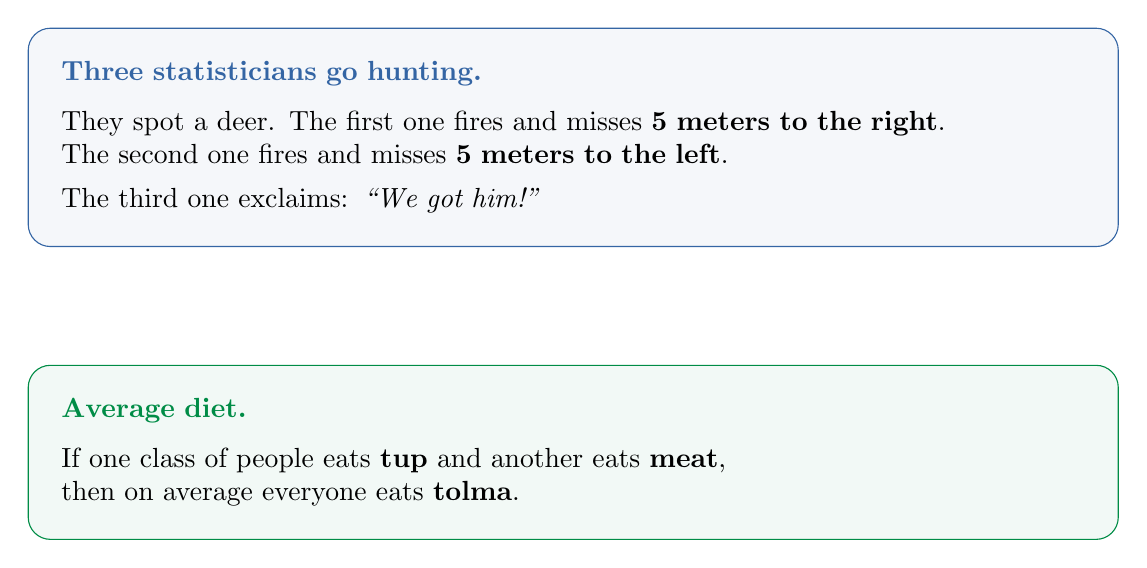
\begin{tikzpicture}
  % Joke 1: Hunters
  \node[draw=popblue, fill=popblue!5, rounded corners=8pt, text width=13cm, align=left, inner sep=12pt] at (0, 2.2) {
    \textbf{\textcolor{popblue}{Three statisticians go hunting.}}\\[6pt]
    They spot a deer. The first one fires and misses \textbf{5 meters to the right}.\\
    The second one fires and misses \textbf{5 meters to the left}.\\[4pt]
    The third one exclaims: \textit{``We got him!''}
  };

  % Joke 2: Tolma
  \node[draw=paramgreen, fill=paramgreen!5, rounded corners=8pt, text width=13cm, align=left, inner sep=12pt] at (0, -1.8) {
    \textbf{\textcolor{paramgreen}{Average diet.}}\\[6pt]
    If one class of people eats \textbf{tup} and another eats \textbf{meat},\\
    then on average everyone eats \textbf{tolma}.
  };
\end{tikzpicture}
\end{center}

\end{frame}

\begin{frame}
\frametitle{Risk and Empirical Risk}
\begin{center}
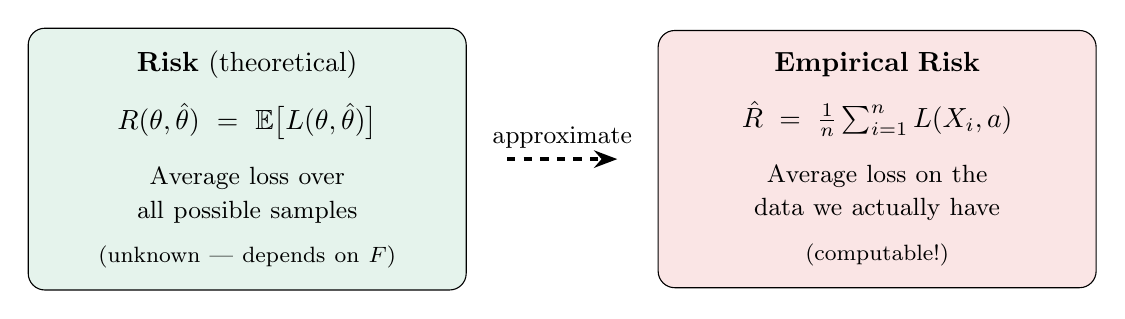
\begin{tikzpicture}[
  riskbox/.style={draw, rounded corners=6pt, minimum width=5.5cm, minimum height=2.5cm, align=center, text width=5cm, inner sep=8pt}
]
  \node[riskbox, fill=paramgreen!10] at (-4, 0) {
    \textbf{Risk} (theoretical)\\[8pt]
    $R(\theta, \hat{\theta}) = \mathbb{E}\bigl[L(\theta, \hat{\theta})\bigr]$\\[8pt]
    {\small Average loss over}\\
    {\small all possible samples}\\[4pt]
    {\footnotesize (unknown --- depends on $F$)}
  };
  \node[riskbox, fill=sampred!10] at (4, 0) {
    \textbf{Empirical Risk}\\[8pt]
    $\hat{R} = \frac{1}{n}\sum_{i=1}^n L(X_i, a)$\\[8pt]
    {\small Average loss on the}\\
    {\small data we actually have}\\[4pt]
    {\footnotesize (computable!)}
  };

  \draw[-{Stealth}, very thick, dashed] (-0.7, 0) -- (0.7, 0)
    node[midway, above, font=\small] {approximate};
\end{tikzpicture}
\end{center}

\vspace{0.5cm}
\textbf{Empirical Risk Minimization (ERM):} choose the estimator that minimizes $\hat{R}$.

\small This principle unifies least squares, maximum likelihood, and most learning algorithms.
\end{frame}

% ============================================================
% ERM AND THE ML CONNECTION
% ============================================================
\section{ERM and the Bigger Picture}

\begin{frame}
\frametitle{ERM in Machine Learning}
\begin{center}
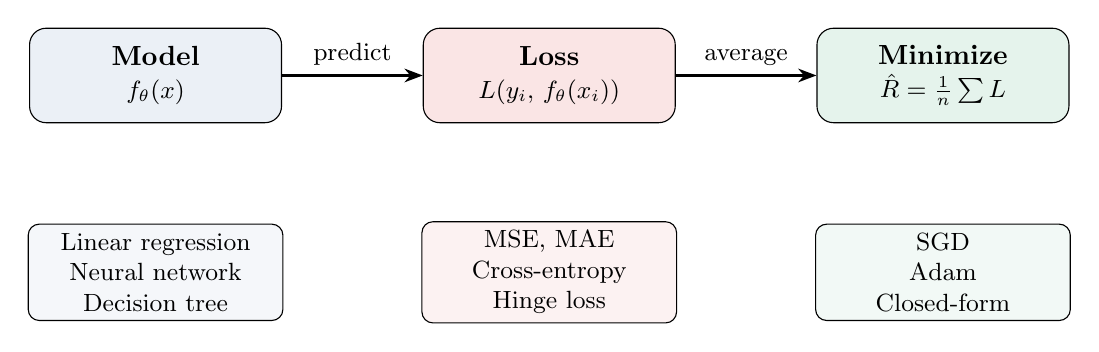
\begin{tikzpicture}[
  stepbox/.style={draw, rounded corners=6pt, minimum width=3.2cm, minimum height=1.2cm, align=center, font=\normalsize, inner sep=6pt}
]
  % The ML pipeline
  \node[stepbox, fill=popblue!10] (model) at (-5, 1) {\textbf{Model}\\{\small $f_\theta(x)$}};
  \node[stepbox, fill=sampred!10] (loss) at (0, 1) {\textbf{Loss}\\{\small $L(y_i,\, f_\theta(x_i))$}};
  \node[stepbox, fill=paramgreen!10] (erm) at (5, 1) {\textbf{Minimize}\\{\small $\hat{R} = \frac{1}{n}\sum L$}};

  \draw[-{Stealth}, thick] (model) -- (loss) node[midway, above, font=\small] {predict};
  \draw[-{Stealth}, thick] (loss) -- (erm) node[midway, above, font=\small] {average};

  % Concrete examples
  \node[draw, rounded corners=4pt, fill=popblue!5, text width=3cm, align=center, font=\small] at (-5, -1.5) {Linear regression\\Neural network\\Decision tree};
  \node[draw, rounded corners=4pt, fill=sampred!5, text width=3cm, align=center, font=\small] at (0, -1.5) {MSE, MAE\\Cross-entropy\\Hinge loss};
  \node[draw, rounded corners=4pt, fill=paramgreen!5, text width=3cm, align=center, font=\small] at (5, -1.5) {SGD\\Adam\\Closed-form};
\end{tikzpicture}
\end{center}

\vspace{0.4cm}
\begin{center}
\fcolorbox{popblue}{popblue!5}{%
  \parbox{11cm}{\centering
    \textbf{Every ML training procedure is ERM.}\\[2pt]
    \small Choose a model class, choose a loss, minimize the empirical risk over parameters.
  }%
}
\end{center}
\end{frame}

\begin{frame}
\frametitle{One Principle, Many Names}
\begin{center}
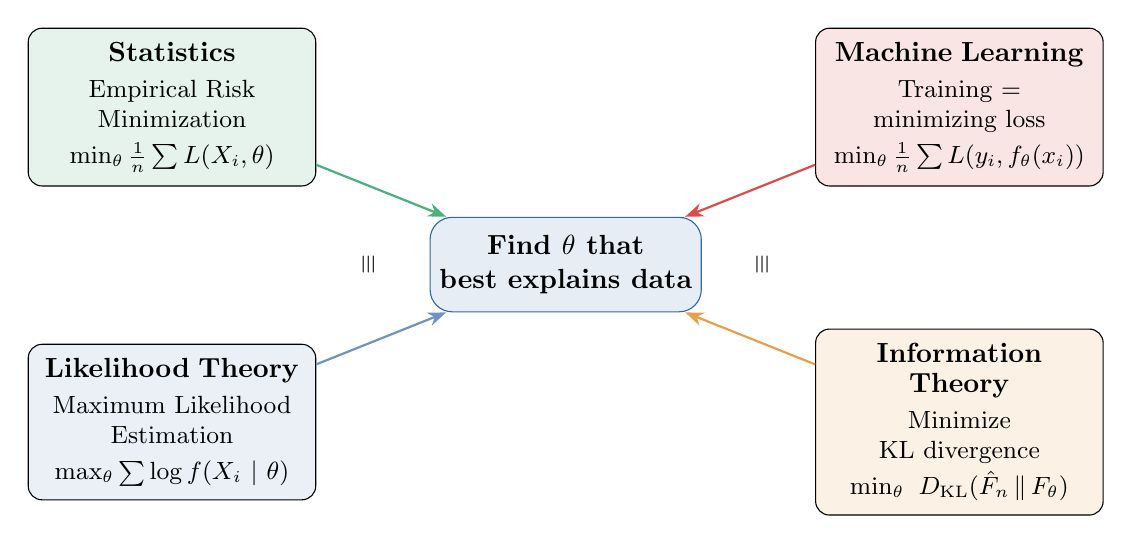
\begin{tikzpicture}[
  unbox/.style={draw, rounded corners=5pt, minimum width=3.5cm, minimum height=1.8cm, align=center, text width=3.3cm, inner sep=5pt, font=\small}
]
  % Central node
  \node[draw=popblue, fill=popblue!12, rounded corners=8pt, minimum width=3cm, minimum height=1.2cm, font=\normalsize\bfseries, align=center] (center) at (0, 0) {Find $\theta$ that\\best explains data};

  % Statistics
  \node[unbox, fill=paramgreen!10] (stat) at (-5, 2) {
    \textbf{\normalsize Statistics}\\[2pt]
    Empirical Risk\\Minimization\\[2pt]
    $\min_\theta \frac{1}{n}\sum L(X_i, \theta)$
  };
  % ML
  \node[unbox, fill=sampred!10] (ml) at (5, 2) {
    \textbf{\normalsize Machine Learning}\\[2pt]
    Training =\\minimizing loss\\[2pt]
    $\min_\theta \frac{1}{n}\sum L(y_i, f_\theta(x_i))$
  };
  % MLE
  \node[unbox, fill=popblue!10] (mle) at (-5, -2) {
    \textbf{\normalsize Likelihood Theory}\\[2pt]
    Maximum Likelihood\\Estimation\\[2pt]
    $\max_\theta \sum \log f(X_i \mid \theta)$
  };
  % Info theory
  \node[unbox, fill=orange1!10] (info) at (5, -2) {
    \textbf{\normalsize Information Theory}\\[2pt]
    Minimize\\KL divergence\\[2pt]
    $\min_\theta \; D_{\text{KL}}(\hat{F}_n \,\|\, F_\theta)$
  };

  \draw[-{Stealth}, thick, paramgreen!70] (stat) -- (center);
  \draw[-{Stealth}, thick, sampred!70] (ml) -- (center);
  \draw[-{Stealth}, thick, popblue!70] (mle) -- (center);
  \draw[-{Stealth}, thick, orange1!70] (info) -- (center);

  % Equivalences on the sides
  \node[font=\small, rotate=90] at (-2.5, 0) {$\equiv$};
  \node[font=\small, rotate=90] at (2.5, 0) {$\equiv$};
\end{tikzpicture}
\end{center}
\vspace{-0.1cm}
{\small\centering MLE with log-loss \textbf{= ERM} with neg.\ log-likelihood \textbf{= minimizing} KL divergence to data.\par}
\end{frame}

\begin{frame}
\begin{center}
  {\Huge\bfseries\textcolor{popblue}{Questions?}}

  \vspace{1cm}

  {\large Next lecture: Descriptive Statistics \& Empirical Distributions}
\end{center}
\end{frame}

\end{document}
